\documentclass[12pt, twoside]{article}
\usepackage[letterpaper, margin=1in, head=30pt, headsep=0.1in]{geometry}
\usepackage[english]{babel}
\usepackage[utf8]{inputenc}
\usepackage{amsmath}
\usepackage{amsfonts}
\usepackage{amssymb}
\usepackage{tikz}
\usetikzlibrary{quotes, angles}

\usepackage{graphicx}
\usepackage{enumitem}
\usepackage{multicol}

%\usepackage{pgfplots}
%\pgfplotsset{width=10cm,compat=1.9}
%\usepgfplotslibrary{statistics}
%\usepackage{pgfplotstable}
%\usepackage{tkz-fct}
%\usepackage{venndiagram}

\usepackage{fancyhdr}
\pagestyle{fancy}
\fancyhf{}
\renewcommand{\headrulewidth}{0pt} % disable the underline of the header
\raggedbottom
\newif\ifmeta
\metatrue %print standards and topics tags

\title{Math AI Worksheet Generator and Formative Assessment System}
\author{Chris Huson}
\date{January 2021}

%\fancyhead[RE]{\thepage}
%\fancyhead[RO]{\thepage \\ Name: \hspace{3cm}}
%\fancyhead[L]{BECA / Dr. Huson / 10th Grade Geometry\\* 7 June 2019}
%
%\begin{document}
%\subsubsection*{13.7 Homework: Cross sections, distance applications}
%\fancyhead[L]{BECA / Dr. Huson / Geometry 03-Volume+angle-bisectors\\* pset ID: 34}

\begin{document}

\subsubsection*{5.4 Rotation}
\begin{enumerate}

\item Do Now: A rotation maps triangle $DEF$ onto triangle $LMN$. \\[0.5cm]
Write the letter or letters for each corresponding object. \vspace{0.5cm}
    \begin{multicols}{2}
      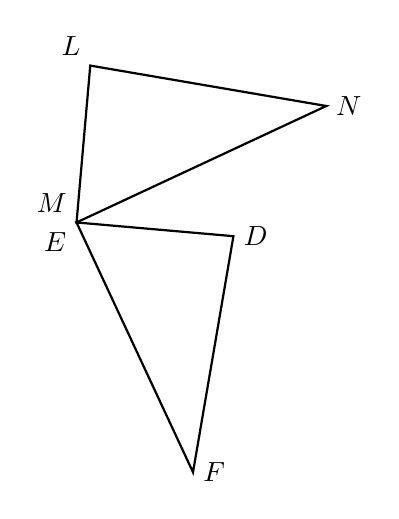
\begin{tikzpicture}[scale=1]
        \coordinate [label=above left:$L$](A) at (85:2);
        \coordinate [label=above left:$M$](B) at (0, 0);
        \coordinate [label=right:$N$](C) at (25:3.5);
        \draw [thick] (A)--(B)--(C)--cycle;
        \draw [thick, rotate=-90] (85:2) node[right]{$D$}--
        (0,0) node[below left]{$E$}--
        (25:3.5) node[right]{$F$}--cycle;
      \end{tikzpicture}

      \begin{enumerate}
        \item $E \rightarrow$ \vspace{1.5cm}
        \item $F \rightarrow$ \vspace{1.5cm}
        \item $DF \rightarrow$ \vspace{1.5cm}
      \end{enumerate}
    \end{multicols}

\newpage
\item Do Now: A rotation centered at the origin maps $A$ to $A'$, as shown, $A(3,1) \rightarrow A'(-1,3)$.
\begin{multicols}{2}
  \begin{enumerate}
    \item Which correctly identifies the rotation?
    \begin{enumerate}[label=(\Alph*)]
      \item Clockwise $180^\circ$
      \item Counter clockwise $180^\circ$
      \item Clockwise $90^\circ$
      \item Counter clockwise $90^\circ$
      \item None of the above
    \end{enumerate} \vspace{2cm}
    %\item What is the horizontal shift, how many squares right or left? \vspace{1.25cm}
    %\item What is the vertical shift, how many squares up or down? \vspace{1.25cm}
    \item If the same translation is applied to $C(5,1)\rightarrow C'(x,y)$, plot and label the point $C'$ as an ordered pair.
    \end{enumerate}
    \begin{flushright}
    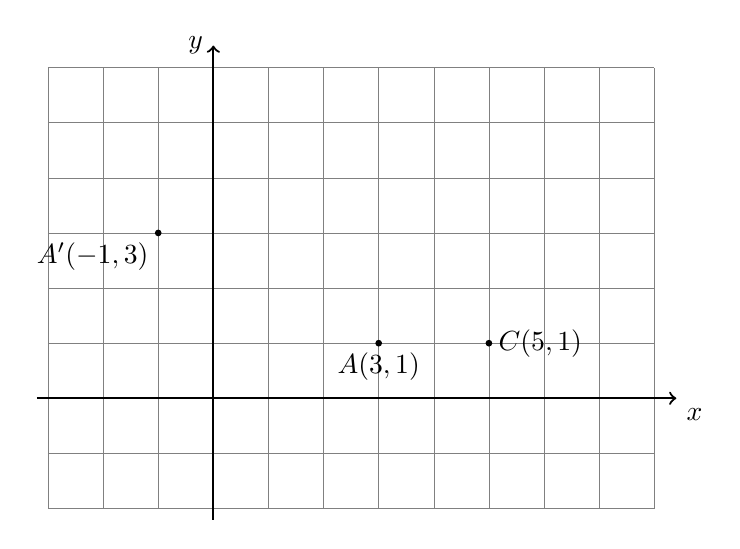
\begin{tikzpicture}[scale=0.7]
      \draw [help lines] (-3,-2) grid (8,6);
      \draw [thick, ->] (-3.2,0) -- (8.4,0) node [below right] {$x$};
      \draw [thick, ->] (0,-2.2)--(0,6.4) node [left] {$y$};
      \draw [fill] (3,1) circle [radius=0.05] node[below] {$A(3,1)$};
      \draw [fill] (-1,3) circle [radius=0.05] node[below left] {$A'(-1,3)$};
      %\draw [->, dashed] (7,1)--(2,3);
      \draw [fill] (5,1) circle [radius=0.05] node[right] {$C(5,1)$};
    \end{tikzpicture}
    \end{flushright}
\end{multicols}

\newpage
\item Rotate the triangle $90^\circ$ clockwise around the origin, $\triangle ABC \rightarrow \triangle A'B'C'$. Complete the table of the coordinates and plot and label the image on the grid. \vspace{0.5cm}
\begin{multicols}{2}
  $A(1,2) \rightarrow$ \\[0.7cm]
  $B(1,4) \rightarrow$ \\[0.7cm]
  $C(4,2) \rightarrow$ \\[0.7cm]
    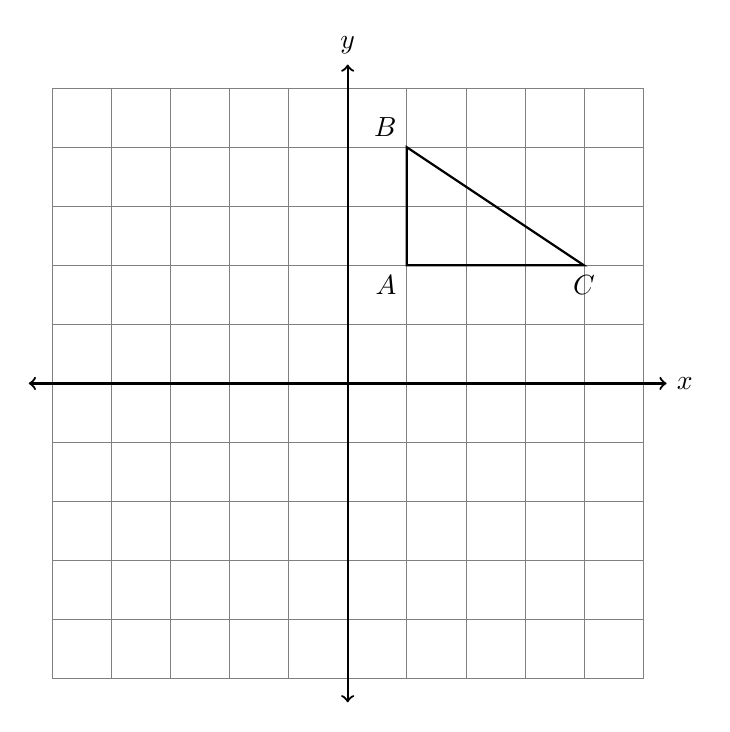
\begin{tikzpicture}[scale=.75]
    \draw [help lines] (-5,-5) grid (5,5);
    \draw [thick, <->] (-5.4,0) -- (5.4,0) node [right] {$x$};
    \draw [thick, <->] (0,-5.4)--(0,5.4) node [above] {$y$};  
    \draw [thick]
      (1,2) node[below left] {$A$}--
      (1,4) node[above left] {$B$}--
      (4,2) node[below] {$C$}--cycle;  
    \end{tikzpicture}
  \end{multicols}

\newpage
\item $\triangle ABC$ is shown with vertices $A(-1,2)$, $B(6,1)$, and $C(5,4)$. Rotate the triangle $90^\circ$ counter clockwise around the origin. Write down its coordinates in a table and plot and label it on the graph.
  \begin{flushright}
    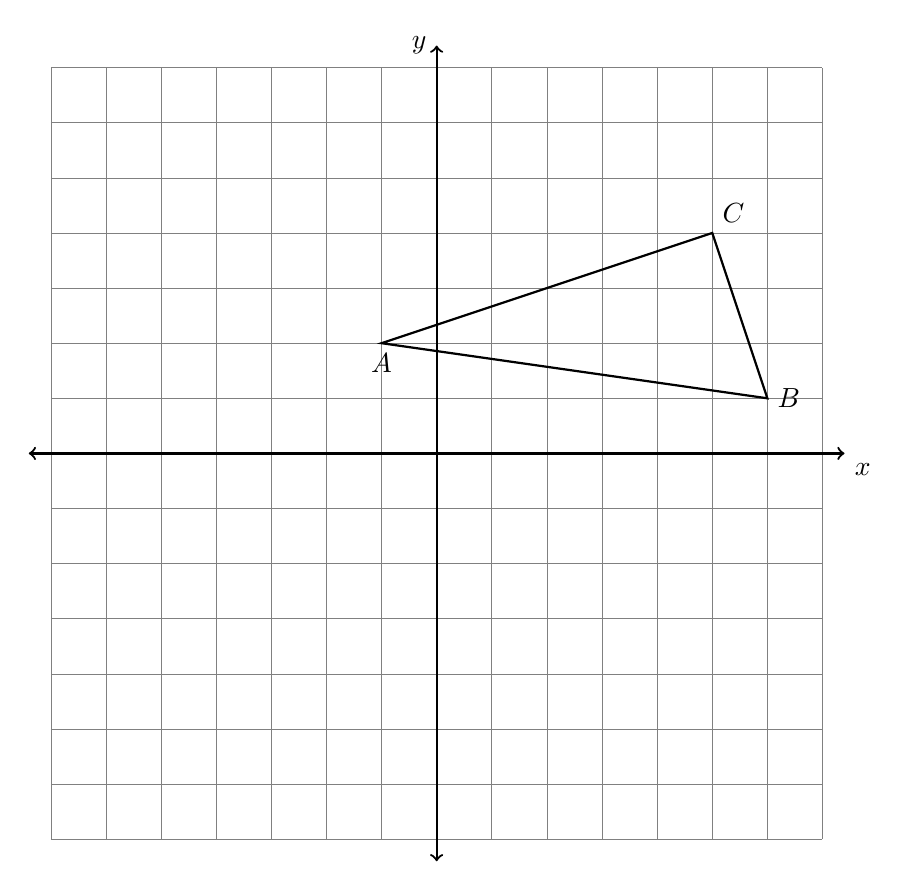
\begin{tikzpicture}[scale=0.7]
      \draw [help lines] (-7,-7) grid (7,7);
      \draw [thick, <->] (-7.4,0) -- (7.4,0) node [below right] {$x$};
      \draw [thick, <->] (0,-7.4)--(0,7.4) node [left] {$y$};
      \draw [thick] (-1,2) node[below] {$A$}--
        (6,1) node[right] {$B$}--
        (5,4) node[above right] {$C$}--
        cycle;
    \end{tikzpicture}
    \end{flushright}


\newpage
\item Do Now: A dilation centered at $A$ maps $\triangle ABC \rightarrow \triangle ADE$. Given that $BC = 8$, $DE = 14$.\\[0.5cm]
Write the value of the scale factor $k$ in the box.
    \begin{flushright}
      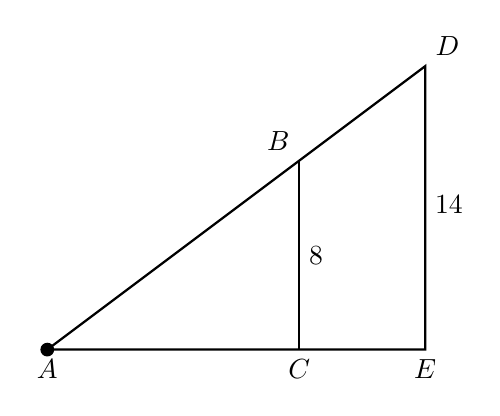
\begin{tikzpicture}[scale=0.8]
        \draw [-, thick] (0,0)--
        (6,0) node[below]{$E$}--
        (6,4.5) node[above right]{$D$}--cycle;
        \draw [thick] (4,0)--(4,3);
        \draw [fill] (0,0) circle [radius=0.1] node[below] {$A$};
        \node at (4,0) [below]{$C$};
        \node at (4,3) [above left]{$B$};
        %\node at (2, 0) [below]{$10$};
        %\node at (2, 2) [above]{$12$};
        \node at (6, 2.3) [right]{$14$};
        \node at (4, 1.5) [right]{$8$};
      \end{tikzpicture}
    \end{flushright}

\newpage
\item Exam review: The perimeter of the isosceles $\triangle FGH$ is $19 \frac{1}{2}$ with $\overline{FH} \cong \overline{GH}$. If $FG=x+2$ and $FH=8 \frac{1}{4}$, find $x$.\\[0.25cm]
    Show your work with an equation.\\[0.5cm]
      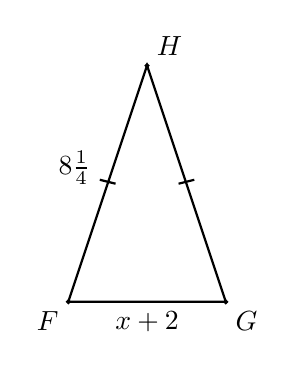
\begin{tikzpicture}[scale=0.5]
        \draw [thick](0,0)--(4,0)--(2,6)--(0,0);
        \draw [fill] (0,0) circle [radius=0.05] node[below left]{$F$};
        \draw [fill] (4,0) circle [radius=0.05] node[below right]{$G$};
        \draw [fill] (2,6) circle [radius=0.05] node[above right]{$H$};
        \draw [thick] (0.8,3.1)--(1.2,3); %tick mark
        \draw [thick] (2.8,3)--(3.2,3.1); %tick mark
        \node at (2,0) [below]{$x+2$};
        \node at (0.8,3.4) [left]{$8 \frac{1}{4}$};
      \end{tikzpicture}
      \begin{flushright}
        Write the value of $x$ in the box.
      \end{flushright}


\end{enumerate}
\end{document}